\section{Chapter 5}
\subsection{Exercises} % Chapter 5
\begin{sol}{Exercise 5.1}
The answer is within the subsequent text.
\end{sol}
\begin{sol}{Exercise 5.2}
There are not many residues in $\mathbb{Z}_7$, so we can just test each manually until we find what we are looking for.
\[
1 \cdot 6 \equiv 6 ~(\text{mod }7)
\]
\[
2 \cdot 6 \equiv 12 \equiv 5 ~(\text{mod }7)
\]
\[
3 \cdot 6 \equiv 18 \equiv 4 ~(\text{mod }7)
\]
\[
4 \cdot 6 \equiv 24 \equiv 3 ~(\text{mod }7)
\]
\[
5 \cdot 6 \equiv 30 \equiv 2 ~(\text{mod }7)
\]
\[
6 \cdot 6 \equiv 36 \equiv 1 ~(\text{mod }7)
\]
and so the multiplicative inverse of $6$ in $\mathbb{Z}_7$ is 6. It is its own inverse!
\end{sol}

\subsection{Problems} % Chapter 5


\begin{sol}{Problem 5.1}
\begin{proof}
Let us denote $\gcd(a,b) = k$. Then, $\exists \alpha, \beta$ such that $a = \alpha k$ and $b = \beta k$ and $\gcd(\alpha, \beta) = 1$ (by definition of the $\gcd(a,b)$ - if this was not 1 then $k$ would not be the greatest common factor). 

Now, we want to find $\gcd(a+b, ab)$. Using the expansions $a = \alpha k$ and $b = \beta k$, we have that
\[
\gcd(a+b, ab) = \gcd(k(\alpha + \beta), k^2\alpha\beta)
\]
\[
= k \cdot \gcd(\alpha + \beta, k\alpha \beta)
\]
and now we focus on the $\gcd(\alpha + \beta, k\alpha \beta)$ term. 

\textbf{Lemma P5.1.1}
\[
\gcd(\alpha, \beta) = 1 \implies\gcd(\alpha + \beta, \alpha \beta) = 1
\]
\begin{proof}
We will proceed by contradiction. Assume $\exists$ a prime $p$ such that $p \mid \alpha \beta$ and $p \mid \alpha + \beta$. Since $p \mid \alpha \beta$, by Euclid's lemma (which requires $\gcd(\alpha, \beta) = 1$ in this case), $p \mid \alpha$ or $p \mid \beta$. 

WLOG, assume $p \mid \alpha$. Since $p \mid \alpha$ and $p \mid \alpha + \beta$, we have that
\[
p \mid (\alpha + \beta) - \alpha \implies p \mid \beta
\]
which directly contradicts Euclid's lemma. Therefore, no prime divides both $\alpha + \beta$ and $\alpha\beta$, and
\[
\gcd(\alpha + \beta, \alpha \beta) = 1
\]
\end{proof}

Now, we are interested in how this relates to $\gcd(\alpha + \beta, k\alpha \beta)$. To do so, we will prove the following lemma. 

\textbf{Lemma P5.1.2}
Given $\gcd(x, y) = 1$
\[
\gcd(x, yz) = \gcd(x, z)
\]
\begin{proof}
Since $x$ and $y$ have no factors in common, any factors $x$ shares with $xz$ must come from $z$, and thus the two quantities are equal since we are essentially searching for the greatest common factor of $x$ and $z$ since $y$ and $x$ have no such factors.
\end{proof}

We now apply this to our current situation
\[
\gcd(\alpha + \beta, k\alpha \beta) = \gcd(\alpha + \beta, k)
\]
and thus the relationship that they are equal is clearly false. However, the relationship between the two terms is as follows (in a somewhat simplified form), substituting all the values we have previously found (i.e. $k = \gcd(a, b)$),
\[
\boxed{\gcd(a+b, ab) = \gcd(a, b) \cdot \gcd\left(\frac{a+b}{\gcd(a, b)}, \gcd(a, b)\right)}
\]
\end{proof}

A long and difficult problem. But the result is very interesting. Perhaps a nicer approach would have been to search for a counterexample to the statement that they are equal. One can be found relatively quickly when $a = b = 2$, leaving the false statement
\[
\gcd(a+b, ab)  = \gcd(2 + 2, 2 \cdot 2) = \gcd (4, 4) = 4
\]
while
\[
\gcd(a, b) = \gcd(2, 2) = 2 \neq 4
\]
after which we can devote effort to disproving/finding the new form.
\end{sol}

\begin{sol}{Problem 5.2}
\begin{proof}
We will first prove a trivial yet useful lemma. 

\textbf{Lemma P5.2.1. }Equal chords lengths imply equal arc lengths.
\begin{proof}
As a general example, consider the below figure. We will aim to prove that
\[
AB = CD \iff \overset{\frown}{AB} = \overset{\frown}{CD}
\]
\begin{center}
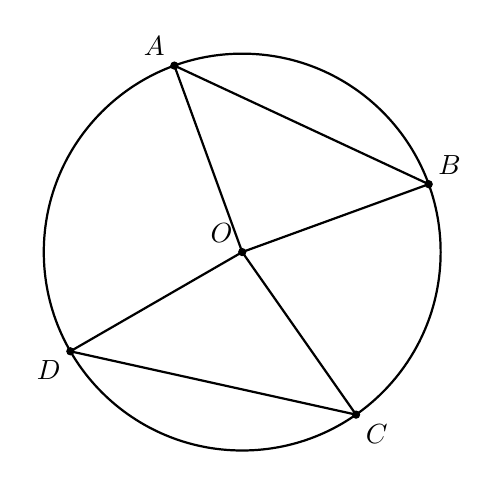
\begin{tikzpicture}[scale=1.8]
  \draw[thick] (0,0) circle (1.4cm);

  \coordinate (A) at (110:1.4);
  \coordinate (B) at (20:1.4);
  \coordinate (C) at (305:1.4);
  \coordinate (D) at (210:1.4);
  \coordinate (O) at (0, 0);

  % Sides
  \draw[thick] (A) -- (B) ;
  \draw[thick] (C) -- (D);

  % Diagonals
  \draw[thick, black] (O) -- (C);
  \draw[thick, black] (O) -- (D);
  \draw[thick, black] (O) -- (A);
  \draw[thick, black] (O) -- (B);

  \filldraw[black] (A) circle (0.025) node[above left]  {$A$};
  \filldraw[black] (B) circle (0.025) node[above right] {$B$};
  \filldraw[black] (C) circle (0.025) node[below right] {$C$};
  \filldraw[black] (D) circle (0.025) node[below left]  {$D$};
  \filldraw[black] (O) circle (0.025) node[above left] {$O$};

\end{tikzpicture}
\end{center}
First, note that since $OA, OB, OC, OD$ are all radii of the circle, we have that
\[
OA = OB = OC = OD
\]
Next, from the definition, we have that $AB = CD$. Therefore, we have the following triangle congruence
\[
\triangle AOB \cong \triangle DOC
\]
by side-side-side (SSS) congruence. Then, since these triangles are congruent, they have congruent corresponding angles. Therefore,
\[
\angle AOB = \angle DOC
\]
and since the measure of an arc is equivalent to the measure of the central angle which subtends that arc,
\[
\overset{\frown}{AB} = \overset{\frown}{CD}
\]
this proves the forwards direction. The backwards direction follows a similar proof, retracing the steps of this proof in that the equal arcs forces equal central angles, and by side-angle-side (SAS) congruence of the triangles, the chords are equal. 
\end{proof}
Consider the below figure.
\begin{center}
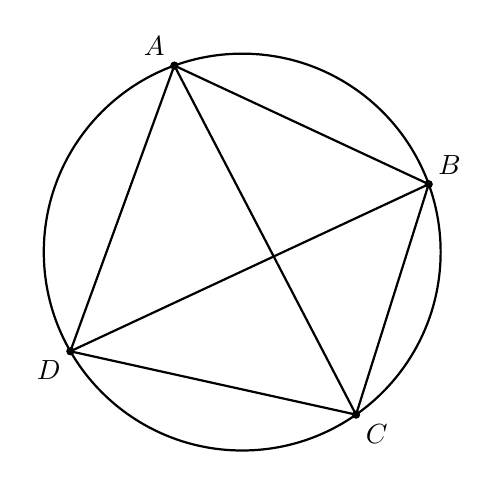
\begin{tikzpicture}[scale=1.8]
  \draw[thick] (0,0) circle (1.4cm);

  \coordinate (A) at (110:1.4);
  \coordinate (B) at (20:1.4);
  \coordinate (C) at (305:1.4);
  \coordinate (D) at (210:1.4);

  % Sides
  \draw[thick] (A) -- (B) -- (C) -- (D) -- cycle;

  % Diagonals
  \draw[thick, black] (A) -- (C);
  \draw[thick, black] (B) -- (D);

  \filldraw[black] (A) circle (0.025) node[above left]  {$A$};
  \filldraw[black] (B) circle (0.025) node[above right] {$B$};
  \filldraw[black] (C) circle (0.025) node[below right] {$C$};
  \filldraw[black] (D) circle (0.025) node[below left]  {$D$};

\end{tikzpicture}
\end{center}
We know now by Lemma P5.2.1 that $\overset{\frown}{AB} = \overset{\frown}{CD}$. Furthermore, we have that chord $AC$ subtends arcs $\overset{\frown}{ADC}$ and $\overset{\frown}{ABC}$. Similarly, chord $BD$ subtends arcs $\overset{\frown}{BAD}$ and $\overset{\frown}{BCD}$. Proving any one of $\overset{\frown}{ADC}$, $\overset{\frown}{ABC}$ is equal to any one of $\overset{\frown}{BAD}$, $\overset{\frown}{BCD}$ proves that chords $AC$ and $BD$ are equal.

Consider arc $\overset{\frown}{BAD}$ subtended by chord $BD$. 
\[
\overset{\frown}{BAD} = \overset{\frown}{AB} + \overset{\frown}{AD}
\]
Similarly, consider arc $\overset{\frown}{ADC}$ subtended by chord $AC$
\[
\overset{\frown}{ADC} = \overset{\frown}{CD} + \overset{\frown}{AD}
\]
and since by Lemma P5.2.1
\[
AB = CD \implies \overset{\frown}{AB} = \overset{\frown}{CD}
\]
we have that 
\[
\overset{\frown}{ADC} = \overset{\frown}{AB} + \overset{\frown}{AD}
\]
and therefore
\[
\overset{\frown}{ADC} = \overset{\frown}{AB} + \overset{\frown}{AD} = \overset{\frown}{BAD}
\]
which by Lemma P5.2.1 implies that
\[
AC = BD
\]
\end{proof}
\end{sol}

\begin{sol}{Problem 5.3}
\begin{proof}
Since $p$ is odd, the set 
\[
\{1, 2, 3, \ldots, p-1\} 
\]
has an even number of members. Thus, we "pair" elements by rearranging the summation
\[
1 + 2 + 3 + \cdots + (p-1) = 
\]
\[
(1 + (p-1)) + (2 + (p-2)) + \cdots + \left(\frac{p-1}{2} + \left(p - \frac{p-1}{2}\right)\right)
\]
such that each pair sums to $p$. We then just have that the sum equates to 
\[
p + p + \cdots + p = \frac{p-1}{2} \cdot p
\]
Therefore, when we take this sum $\pmod{p}$, we get
\[
\frac{p-1}{2} \cdot p \equiv 0 \pmod{p}
\]
since $p \mid \frac{p-1}{2} \cdot p$. Now, we prove the second statement. Since $1 \cdot 2 \cdots (p-1)$ is, by definition $(p-1)!$, we basically want to prove that
\[
(p-1)! \equiv -1 \pmod{p}
\]
which is true by Wilson's Theorem (we use a pairing argument, and we are left with 1 and $p-1$ as the final pair which multiply to $-1 \pmod{p}$). 
\end{proof}
\end{sol}

\begin{sol}{Problem 5.4}
\begin{proof}
Consider the following diagram.
\begin{center}
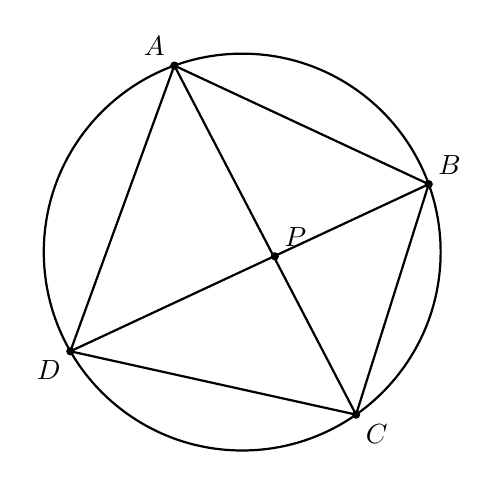
\begin{tikzpicture}[scale=1.8]
  \draw[thick] (0,0) circle (1.4cm);

  \coordinate (A) at (110:1.4);
  \coordinate (B) at (20:1.4);
  \coordinate (C) at (305:1.4);
  \coordinate (D) at (210:1.4);
  \coordinate (P) at (.23, -.03);

  % Sides
  \draw[thick] (A) -- (B) -- (C) -- (D) -- cycle;

  % Diagonals
  \draw[thick, black] (A) -- (C);
  \draw[thick, black] (B) -- (D);

  \filldraw[black] (A) circle (0.025) node[above left]  {$A$};
  \filldraw[black] (B) circle (0.025) node[above right] {$B$};
  \filldraw[black] (C) circle (0.025) node[below right] {$C$};
  \filldraw[black] (D) circle (0.025) node[below left]  {$D$};
  \filldraw[black] (P) circle (0.025) node[above right]  {$P$};

\end{tikzpicture}
\end{center}

First, we prove that $\triangle APB \sim \triangle DPC$. We do this via AA similarity. First note that $\angle APB = \angle DPC$ by the vertical angle theorem (this is nothing special, it is visually intuitive that these angles are equal since they are mirror images of each other). 

Next, we use the result that inscribed angles that subtend the same arc are of the same measure. By this result,
\[
\angle BAP = \angle BAC = \angle CDB = \angle CDP
\]
and since we have two sets of congruent angles, by angle-angle similarity, we have that
\[
\triangle APB \sim \triangle DPC
\]

Next, we prove that $\triangle APD \sim \triangle BPC$. First, note that by vertical angle theorem $\angle APD = \angle BPC$. Next, by the result that inscribed angles that subtend the same arc have the same measure, $\angle DAP = \angle DAC = \angle CBD = \angle CBP$, and by angle-angle similarity we thus have
\[
\triangle APD \sim \triangle BPC
\]
Now we prove the Power of a Point formula. (Note that we don't even need the second similar triangle example to prove this.) Consider $\triangle APB \sim \triangle DPC$. We have that, due to similarity,
\[
\frac{AP}{DP} = \frac{BP}{CP}
\]
cross-multiplying gives us
\[
AP \cdot CP = BP \cdot DP
\]
and simply flipping the terms makes it more clear
\[
PA \cdot PC = PB \cdot PD
\]
that for a point in the center, we may draw intersecting chords through the point with endpoints on the circle, and that for any two such chords $AC$ and $BD$, the following holds true.
\end{proof}
\end{sol}

\begin{sol}{Problem 5.5}
\begin{proof}
We start with Wilson's theorem, a known fact.
\[
(p-1)! \equiv -1 \pmod{p}
\]
\[
(p-1) \cdot (p-2) \cdots 2 \cdot 1 \equiv -1 \pmod{p}
\]
Rearranging the left-hand-side, we get
\[
(p-1)! \equiv 
\]
\[
1 \cdot 2 \cdots \frac{p-1}{2}\cdot (p-1) \cdot (p-2) \cdots \left(p - \frac{p-1}{2}\right) \equiv -1\pmod{p}
\]
Then, we use the fact that $p - k \equiv -k \pmod{p}$ since $p \equiv 0 \pmod{p}$.
\[
1 \cdot 2 \cdots \frac{p-1}{2}  \cdot (-1) \cdot (-2) \cdots \left(-\frac{p-1}{2}\right) \equiv -1\pmod{p}
\]
\[
\left(\frac{p-1}{2}\right)! \cdot (-1)^{\frac{p-1}{2}} \left(\frac{p-1}{2}\right)! \equiv -1\pmod{p}
\]
\[
(-1)^{\frac{p-1}{2}}\left(\left(\frac{p-1}{2}\right)!\right)^2 \equiv -1 \pmod{p}
\]
Note that the inverse of $-1$ in $\mathbb{Z}_p$ is always itself; $-1 \cdot -1 \equiv 1 \pmod{p}$. Thus, we multiply both sides by the inverse of $(-1)^{\frac{p-1}{2}}$, namely, we multiply both sides by $(-1)^{\frac{p-1}{2}}$ itself.
\[
(-1)^{\frac{p-1}{2}} \cdot (-1)^{\frac{p-1}{2}}\left(\left(\frac{p-1}{2}\right)!\right)^2 \equiv (-1)^{\frac{p-1}{2}}\cdot -1 \pmod{p}
\]
\[
\left(\left(\frac{p-1}{2}\right)!\right)^2 \equiv (-1)^{\frac{p-1}{2}}\cdot -1 \pmod{p}
\]
and thus we simply add the exponents
\[
\left(\left(\frac{p-1}{2}\right)!\right)^2 \equiv (-1)^{\frac{p-1}{2} + 1} \pmod{p}
\]
and since $\frac{p-1}{2} + 1 = \frac{p-1}{2} + \frac{2}{2} = \frac{p+1}{2}$, we have that
\[
\left(\left(\frac{p-1}{2}\right)!\right)^2 \equiv (-1)^{\frac{p+1}{2}} \pmod{p}
\]
\end{proof}
\end{sol}

\begin{sol}{Problem 5.6}
Recall from chapter 3 the key result that
\[
a - b \mid P(a) - P(b)
\]
for all integers $a, b$ and polynomials $P(x)$ with integer coefficients ($P \in \mathbb{Z}[x]$). This will be a key result we use in this proof.
\begin{proof}
We assume for contradiction that there exists a function $P(x)$ with degree $\geq 1$ such that $\forall x \geq 1$, $P(x)$ is a prime. Then, consider a fixed $a \geq 1$. $P(a)$ must be a prime number, we will denote it $p_a$; $P(a) = p_a$. By theorem (3.3), we have that
\[
(a + kp_a) - a \mid P(a + kp_a) - P(a)
\]
which simplifies to 
\[
(k-1)p_a \mid P(a + kp_a) - p_a
\]
and therefore, 
\[
P(a + kp_a) - (k-1)p_a \equiv 0 \pmod{p_a}
\]
and since $p_a \equiv 0 \pmod{p_a}$, we get
\[
P(a + kp_a) \equiv 0 \pmod{p_a}
\]
and since $P(x)$ is always prime, we have $P(a + kp_a) = p_a$. However, note that for any number $k$, we must have that $P(a + kp_a)$ must be $p_a$, else we get a contradiction. Thus, for all infinitely many $k \in \mathbb{Z}$, $P(a + kp_a) = p_a$. 

Now, consider polynomial $Q(x) = P(x) - p_a$.
\[
Q (a  + kp_a) = 0 \quad \forall k \in \mathbb{Z}
\]
and therefore this function has infinitely many roots. Thus, there exist infinitely many $q_1, q_2, \ldots$ such that
\[
Q(q_k) = 0 \quad \forall k
\]
and so 
\[
Q(x) = \alpha (x - q_1)(x-q_2)\cdots
\]
which is an infinite sequence, giving the polynomial infinitely large degree. A polynomial cannot have an infinitely large degree, or be represented by an infinite sequence, since by definition, a polynomial must have a finite number of terms. This is a contradiction, and thus, no such polynomial $P(x)$ can exist.
\end{proof}

This is a brief look at a principle we call "infinite descent" or "infinite ascent" (depending on which way we go), which is very useful in contradiction cases like these to show there are infinitely many of something. We will see more of this in Volume 2. 
\end{sol}

\begin{sol}{Problem 5.7}
This is a trick question!
\begin{proof}
Consider the example, $n = 2$, $a_1 = 2, a_2 = 1$. We have
\[
(a_1-1)(a_2-2) = (2-1)(1-2) = (1)(-1) = -1
\]
which is not even. This is a counterexample, and thus the statement is false.
\end{proof}
The moral of the story is don't believe the statement is true just because I told you so! You should usually check with some dummy numbers and cases to a) check if it is true and b) get a better feel for the problem at hand. In this case, a counterexample was very easy to find. 
\end{sol}

\begin{sol}{Problem 5.8}
\begin{proof}
We proceed by splitting this into two separate proofs, by the result that if $\gcd(p,q) = 1$, then $a \equiv 0 \pmod{pq}$ implies that $a \equiv 0 \pmod{p}$ and $a \equiv 0 \pmod{q}$. We thus prove these separately.

Beginning with the proof of $\pmod{p}$. Consider
\[
4((p-1)!+1)+p \equiv 4((p-1)!+1) \pmod{p}
\]
Then, by Wilson's theorem
\[
4((p-1)!+1) \equiv 4(-1+1) \equiv 4 \cdot 0 \equiv 0 \pmod{p}
\]
which proves that
\[
4((p-1)!+1)+p \equiv 0 \pmod{p}
\]

Next, we consider the proof of equivalence to 0 $\pmod{q}$. Since $q = p+2$, we check $\pmod{(p+2)}$. First, we will rewrite the terms. $p \equiv -2 \pmod{(p+2)}$. Furthermore, we have that
\[
(p+1)(p)(p-1)! = (p+1)!
\]
and since by Wilson's Theorem, $(p+1)! \equiv -1 \pmod{(p+2)}$, we get that
\[
(p+1)(p)(p-1)! \equiv -1 \pmod{(p+2)}
\]
note that $p = (p+2)-2$ and $p+1 = (p+2)-1$, so we have that
\[
(-1)(-2)(p-1)! \equiv -1 \pmod{(p+2)}
\]
and so 
\[
2 (p-1)! \equiv -1 \pmod{(p+2)}
\]
which implies that
\[
4 (p-1)! \equiv -2 \pmod{(p+2)}
\]
We use this to substitute into the original equation.
\[
4((p-1)! + 1) + p \equiv 4(p-1)! + 4 -2 \pmod{(p+2)}
\]
\[
4(p-1)! + 4 -2 \equiv -2 + 4 -2 \equiv 0\pmod{(p+2)} 
\]
and since $q = p+2$,
\[
4((p-1)! + 1) + p \equiv 0 \pmod{q}
\]
since it is congruent to 0 both $\pmod{q}$ and $\pmod{p}$, we have that
\[
4((p-1)! + 1) + p \equiv 0 \pmod{pq}
\]
\end{proof}
This result is known as Clement's Theorem.
\end{sol}

\begin{sol}{Problem 5.9}
Before we begin the proof, we will note that for any integer 
\[
a = p_1^{e_1}p_2^{e_2}\cdots p_n^{e_n} = \prod_{i=1}^{n}p_e^{e_i}
\]
the sum of all of its divisors is 
\[
s(a) = (1 + p_1  + \cdots + p_1^{e_1})(1 + p_2  + \cdots p_2^{e_2}) \cdots (1 + p_n + \cdots + p_n^{e_n})
\]
\[
= \prod_{i=1}^{n}{\left(\sum_{j=0}^{e_i}{p_i^j}\right)}
\]
and so the sum of its proper divisors is 
\[
s(a) - a
\]
\begin{proof}
Let $p := 2^k - 1$ be prime. Then, 
\[
n = 2^{k-1} \cdot p = 2^{k-1} \cdot p^1
\]
which has 
\[
s(n)-n = (1 + 2 + 4 + \cdots + 2^{k-1})(1 + p) - 2^{k-1} \cdot p
\]
and now we substitute back $p := 2^k - 1$ (we used this so we could better see how the formula for $s(n)$ was used). 
\[
s(n) - n = (1 + 2 + \cdots + 2^{k-1})(2^k) - (2^{2k-1} - 2^{k-1}) 
\]
\[
= 2^k \left(\sum_{i=0}^{k-1}{2^i}\right) - 2^{2k-1} + 2^{k-1}
\]
\[
= \sum_{i=k}^{2k-1} {2^i}- 2^{2k-1} + 2^{k-1} =  \sum_{i=k}^{2k-2} {2^i} + 2^{k-1}
\]
We now factor out the $2^{k-1}$ (and shift the indices of the summation accordingly)
\[
= 2^{k-1}\left(  \sum_{i=1}^{k-1}{2^i} + 1 \right) = 2^{k-1}\left(  \sum_{i=0}^{k-1}{2^i}\right)
\]
and now we use the identity that
\[
1 + 2 + 4 + \cdots + 2^{k-1} = 2^k -1
\]
\[
2^{k-1}\left(  \sum_{i=0}^{k-1}{2^i}\right) = 2^{k-1} \cdot (2^k-1) = n
\]
and thus we found that
\[
s(n)-n=n
\]
which proves that $n$ is a perfect number.
\end{proof}
\end{sol}

\begin{sol}{Problem 5.10}
First, we will prove that 
\[
p \mid {\binom{p}{k}} \quad \forall k \in [1, p-1]
\]
\begin{proof}
By definition, 
\[
{\binom{p}{k}} = \frac{p!}{k!(p-k)!}
\]
and since $k < p$ and $p-k < p$ (since $k \neq 0$ and $k \neq p$), we have that the numerator will always have a factor of $p$. We can be certain since $p$ is prime, there does not exist any number less than $p$ which divides $p$ (other than 1, but $p/1 = p$). 
\end{proof}
Now, we will prove the main theorem, which looks like an mistake we make in school, but is in fact a true statement (no tricks this time).
\begin{proof}
By the Binomial Expansion, 
\[
(n+m)^p = \sum_{i=0}^{p}{{\binom{10}{0}}n^{p-i}m^{i}}
\]
\[
= {\binom{10}{0}}n^p + {\binom{10}{1}}n^{p-1}m + \cdots + {\binom{10}{}10}m^p
\]
and since $p \mid {\binom{p}{k}},  k \in [1, p-1]$, all the middle terms are congruent to $0 \pmod{p}$. Every term except the first and last has a factor of $p$, and is therefore equivalent to 0. Thus, when we take the $\pmod{p}$ of both sides, we get
\[
{\binom{10}{0}}n^p + 0 \cdots + {\binom{10}{10}}m^p \equiv n^p + m^p \pmod{p}
\]
which proves the result.
\end{proof}
\end{sol}

\begin{sol}{Problem 5.11}
\begin{proof}
We begin by checking small primes.
$p = 2$:
\[
2^2 + 2 = 6
\]
which is not a prime.

$p = 3$
\[
3^2 + 2 = 1
\]
which is indeed prime. Now, after checking a few more small primes, we find no other solutions. Thus, we switch to a general approach. Assume for contradiction there exists a prime $p > 3$ such that $p^2 + 2$ is also prime. Since $p$ is a prime greater than 3, 
\[
p \equiv 1, 2 \pmod{3}
\]
and thus 
\[
p^2 \equiv 1 \pmod{3}
\]
However, this means that 
\[
p^2 + 2 \equiv 3 \equiv 0 \pmod{3}
\]
which implies that $3 \mid p^2 + 2$ for all $p > 3$. This contradicts that $p^2 + 2$ is a prime number, since it is divisible by 3 and greater than 3. Therefore, the only solution is 
\[
\boxed{\begin{cases}p=3 \\p^2 + 2 = 11\end{cases}}
\]
\end{proof}
\end{sol}

\begin{sol}{Problem 5.12}
\begin{proof}

Consider the following diagram.

We will first prove that 
\[
\frac{b}{\sin B } = 2R
\]
and note that the proof for the other two angle-side pairs follow the same, up to symmetry. 

First, we will draw a diameter from point $A$ and label the center of the circumcircle $O$ and the antipode of $A$ (the point across from the diameter) as $D$. 

\begin{center}
\begin{tikzpicture}[scale=2]

% Circle
\draw[thick] (0,0) circle (1.5);

% Center
\coordinate (O) at (0,0);

% Triangle vertices
\coordinate (A) at (100:1.5);
\coordinate (B) at (210:1.5);
\coordinate (C) at (20:1.5);

% Point D opposite A (diameter)
\coordinate (D) at ($(O)!-1!(A)$);

% Triangle
\draw[thick] (A)--(B)--(C)--cycle;

% Diameter
\draw[dashed] (A)--(D);

% Extra side
\draw[thick] (C)--(D);

% Labels
\fill (A) circle (0.025) node[above] {$A$};
\fill (B) circle (0.025) node[below left] {$B$};
\fill (C) circle (0.025) node[right] {$C$};
\fill (D) circle (0.025) node[below] {$D$};
\fill (O) circle (0.02) node[left] {$O$};

\end{tikzpicture}
\end{center}
Note that $AD = 2R$. We have also drawn $CD$, which together all form $\triangle ACD$. Since $AD$ is a diameter, the inscribed angle of the diameter, $\angle ACD$, is a right angle. 

Then, since $\angle ABC$ and $\angle CDA$ subtend the same arc, we have that
\[
\angle B = \angle ABC = \angle CDA
\]
Then, 
\[
\sin(\angle CDA) = \frac{AC}{AD} = \frac{AC}{2R}
\]
and by the equality, we have
\[
\sin B = \frac{AC}{2R}
\]
by convention, $b$ is the side opposite of angle $B$. Thus, $b = AC$. 
\[
\sin B = \frac{b}{2R}
\]
and rearranging gives us
\[
\frac{b}{\sin B} = 2R
\]
The proofs for the other angle-side pairs follow the same, drawing in diameters from the other points and using the same reasoning.
\end{proof}
\end{sol}

\begin{sol}{Problem 5.13}
This problem was inspired, in part, by the Ross mathematics program and some of the application problem sets. While still perhaps a little easier (this is subjective!), I hope it carried through the spirit of the problem to endure and stay curious!

Part (a).
\begin{proof}
\[
2 \star 3 = 2 + 3 + 2 \cdot 3 = 2 + 3 + 6 = 11
\]
\[
3 \star 5 = 3 + 5 + 3 \cdot 5 = 23
\]
\[
0 \star a = 0 + a + 0 \cdot a = a
\]
$0$ acts like the identity element since $0 \star a = a \star 0 = a$ for all $a \in \mathbb{R}$. 
\end{proof}
Part (b).
\begin{proof}
\[
a \star x = 0
\]
\[
a + x + ax = 0
\]
\[
ax + a + x + 1 = 1
\]
\[
(a+1)(x+1) = 1
\]
\[
x+1 =\frac{1}{a+1}
\]
\[
\boxed{x = -\frac{a}{a+1}}
\]
A solution exists for all $a \neq -1$.
\end{proof}
The method of adding 1 and factoring the expression is a common Olympiad technique known as Simons's Favorite factoring Trick (SFFT), and is very useful in factoring expressions of the above form. 
Part (c).
\begin{proof}
First note that the operation is not distributive across addition. (This lemma is not necessary for the proof, but this is an exploration. The more we explore the better!)

\textbf{Lemma P5.13.1}
\[
(a+b) \star c \neq a \star c + b \star c
\]
\begin{proof}
\[
(a+b) \star c = (a+b) + c + (a+b)c = a + b + c + ac + bc
\]
Meanwhile,
\[
a \star c + b \star c = a + c + ac + b + c + bc
\]
\[
= a + b + 2c + ac + bc
\]
and clearly these two are not equal.
\end{proof}

Consider the left-hand side,
\[
(a \star b) \star c = (a + b + ab) \star c
\]
since the $\star$ is not distributive over addition, we must treat $a + b + ab$ as a single term.
\[
= (a + b + ab) + c + c(a + b + ab)
\]
\[
 = a + b + c + ab + ac + bc + abc
\]
Now, for the right hand side.
\[
a \star (b \star c) = a \star (b + c + bc)
\]
\[
= a + (b + c + bc) + a(b + c + bc)
\]
\[
= a + b + c + ab + ac + bc + abc
\]
and since they both equal the same expression, 
\[
(a \star b) \star c = a \star (b \star c)
\]
for all real numbers. Therefore, the $\star$ operation is associative.
\end{proof}

Part (d).
\begin{proof}
\[
f(a \star b) = 1 + (a \star b) = 1  + a + b + ab
\]
Then,
\[
f(a)f(b) = (1+a)(1+b) = 1 +a + b + ab
\]
since they are both equal to the same thing, they are equal to each other
\[
f(a \star b) = 1 + (a \star b) = 1  + a + b + ab = f(a)f(b)
\]
\end{proof}

Part (e).
\begin{proof}
We use the associative property to rewrite this as 
\[
(\cdots ((a_1 \star a_2) \star a_3) \cdots ) \star a_n = x
\]
for some $x \in \mathbb{R}$. Now, take $f(x)$ of both sides:
\[
f\big((\cdots ((a_1 \star a_2) \star a_3) \cdots ) \star a_n\big) = x+1.
\]
We now apply the identity recursively:
\[
f\big((\cdots ((a_1 \star a_2) \star a_3) \cdots ) \star a_n\big)
\]
\[
= f\big((\cdots ((a_1 \star a_2) \star a_3) \cdots )\big)\,f(a_n)
\]
which we can keep applying until we reduce the equation into
\[
((\ldots ((a_1 \star a_2) \star a_3) \ldots ) \star a_n) = f(a_1)f(a_2)\cdots f(a_n)
\]
\[
= \prod_{i=1}^{n}{f(a_i)}
\]
Recall the original equation, and substituting this simplified form, we get
\[
\prod_{i=1}^{n}{f(a_i} = x + 1
\]
and since $f(x) = x + 1$
\[
\prod_{i=1}^{n}{(a_i+1)} = x + 1
\]
and so the repeated $\star$ expression is 
\[
x = \boxed{\prod_{i=1}^{n}{(a_i+1)}  - 1}
\]
\end{proof}

Part (f).
\begin{proof}
We use the previous result
\[
x^{\star n} = (x+1)^n - 1
\]
Since we want $x^{\star n} = x$, we have
\[
(x+1)^n - 1 = x
\]
\[
(x+1)^n = x + 1
\]
\[
(x+1)^{n-1} = 1
\]
After which there are two cases. First, $x= 0$. 
\[
x = 0 \implies (x+1)^{n-1} = 1^{n-1}
\]
which is equal to $1$ for any $n$. Thus, any pair of the form $(0, n)$ is a solution. 

The second case is $x = -2$. 
\[
x = -2 \implies (x+1)^{n-1} = (-1)^{n-1}
\]
which is equal to $1$ for any even $n-1$; which corresponds to odd $n$. Thus, any $n$ of the form $2k + 1, k \geq 0$ forms a solution $(-2, 2k+1)$.
\end{proof}

Part (g.a).
There is not much "proving" to be done here, so use this as a place to check if your calculations are correct. The sequence is:
\[
0, 1, 1, 3, 7, 31, 255, 8191, \ldots
\]

Part (g.b)
Since $f(x) = x + 1$, we just add one to each term.
\[
0, 2, 2, 4, 8, 32, 256, 8192
\]
notice something interesting?

Part (g.c)
\begin{proof}
We begin with a heuristic observation. The sequence
\[
0, 1, 1, 3, 7, 31, 255, 8191, \ldots
\]
can be rewritten
\[
2^0 - 1, 2^1 - 1, 2^1 - 1, 2^2 - 1, 2^3 - 1, 2^5 - 1, 2^8 - 1, 2^{13}-1 \ldots
\]
and we notice that the exponents form the regular Fibonacci sequence. We thus conjecture that the $k$-th term of the sequence is 
\[
s_k = 2^{F_k}-1
\]
where $F_k$ is the $k$-th term of the Fibonacci sequence. We now set out to prove this. Consider the $f-\star$-nacci sequence 
\[
2^0, 2^1, 2^1, 2^2, 2^3, 2^5, 2^8, 2^{13}, \ldots
\]
Each term in this sequence is defined as follows
\[
f(s_k) = f(s_{k-1})f(s_{k-2})
\]
and so each term is the product of the two previous terms. We will consider this full sequence $\log_2$.  Multiplication of numbers corresponds to addition of the powers. In this $\log_2$-$f$-$\star$-nacci sequence, the multiplicative rule becomes additive, such that each term 
\[
\log_2(f(s_k)) = \log_2(f(s_{k-1})) + \log_2(f(s_{k-2}))
\]
which is the rule of the Fibonacci sequence. Thus, the sequence 
\[
\log_2(f(s_{k}))\ = F_k
\]
behaves like the Fibonacci sequence. Thus, undoing this, we have that 
\[
f(s_{k}) = 2^{F_k}
\]
\[
s_k + 1 = 2^{F_k}
\]
\[
s_k = 2^{F_k}-1
\]
which is our original $\star$-nacci sequence.
\end{proof}

Part (h).
What are some questions? One question would be to explore the general formula for the $\star$-nacci sequence for general $s_0$, $s_1$. You could explore more about the $a^{\star n}$ structure, let's call it $\star$-ponent. For which $\star$-ponents do sequences like 
\[
a^{\star1}, a^{\star2}, \ldots
\]
converge to a finite value? What about an infinite value? Is there a clean explicit formula for the sum of these sequences? Is there a well-defined $a^{\star -n}$? Try to define a negative $\star$-ponent that makes sense (i.e. $a^{\star -n} \star a^{\star n} = 0$. Of course, there are much more questions one could ask and explore. Essentially, you can formulate any question by replacing traditional multiplication with the $\star$ operation and seeing how things react. Have fun exploring!
\end{sol}
